
\subsection{Path injections}

\begin{figure}
	\centering
	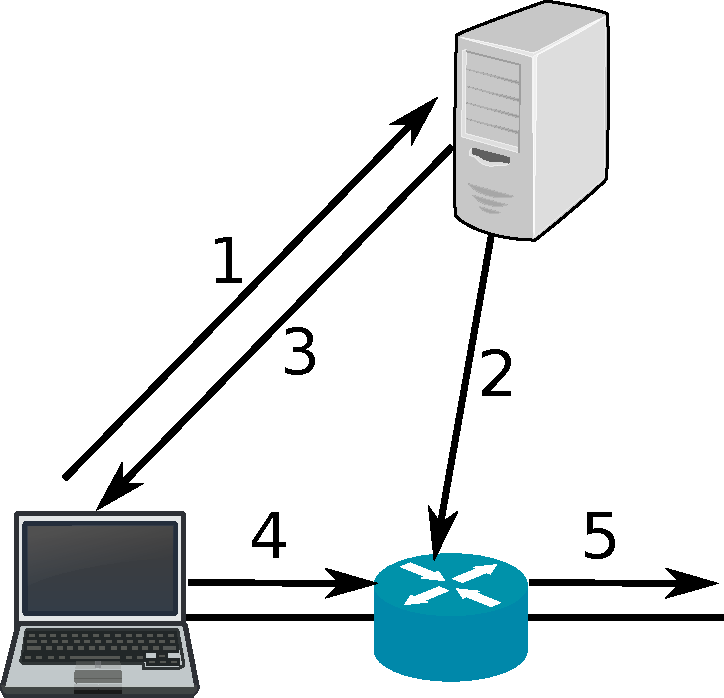
\includegraphics[width=0.5\columnwidth]{figs/controller_communication.pdf}
	\caption{Endhost path query to the controller.}
	\label{fig:path-injection}
\end{figure}

This paper proposes to integrate TCP with SRv6 to optimise congestion.
We reuse a similar controller as in Software Resolved Networks \cite{srn}.
As shown in Figure \ref{fig:path-injection}, an application on the endhost
can query (1) the controller for a path to reach a particular destination.
The SRN query is implemented by extending DNS requests.
The controller computes a path, build its SRH and assign it a binding segment,
that we call Path ID.
After compuation, the mapping between the binding segment and the SRH is inserted
in the access router (2). Then, the controller sends the Path-ID inside the DNS reply
back to the endhost (3). The application can then build an SRH containing only the Path-ID
and insert it in all its packets (4). The access router reads the Path-ID and encapsulate
the packet in an outer IPv6 packet with an SRH that steer the packet through the actual path.

While this first prototype shows that we can build a SDN solution with SRv6,
this prototype has two issues. First, it requires to modify applications to talk
to a controller. This raises deployment issues if you want to control the path taken by
all your applications. Second, it did not consider reaction to congestion, only to failures.

In this paper, we offload the choice of the path to the endhost. The TCP stack of endhosts have
access to the congestion state of each connection. This state, along with information from the
controller enables the endhost to choose between paths that it received from the controller.

We extend the solution by enabling a daemon, the Path Daemon\todo{name ?},
in endhosts to request for a set of dijsoint paths.
The path are disjoint so that we know that a congestion occuring on a path does not influence
the others. The endhost can remain agnostic of the actual topology of the network and it
will not waste time hitting paths that suffer from congestion on the same link.

We use \todo{insert algo name ???} from \cite{aubry2015traffic} to find these disjoint paths.
This algorithm is specific
to SRv6 because it compute disjoint paths between two endpoints and checks that these paths can be expressed
in fewer segments than a given limit. Some hardware components in their network
do not support arbitrarily long SRHs as documented in \cite{sr-hardware-segment-limit}.

The controller computes a set of disjoint paths for every set of pair of source prefix/destination prefix.
Each endhost daemon receives a list of Path IDs for pairs matching its access router as source.
Along with the Path ID, the controller sends the bandwidth capacity, its current usage and its delay.
We scales up the number of controllers with the number of endhost
\todo{inaccurate, it is actually the database but it might be simpler to explain that}.

\subsection{Application-independent path management}

\begin{figure}
	\centering
	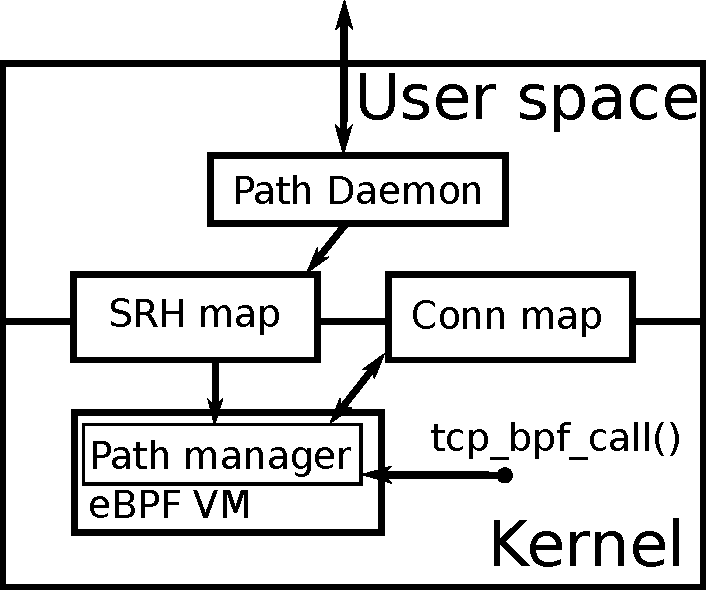
\includegraphics[width=0.5\columnwidth]{figs/ebpf_representation.pdf}
	\caption{Path management code talks through eBPF maps to the Path Daemon.}
	\label{fig:ebpf-representation}
\end{figure}

The previous section describes the path injection to a daemon that runs on the endhost.
However this endhost needs to enable other applications to manage these paths without actually modifying them.
A solution could be to modify the kernel directly to include this path management.
However, this would require operators to modify the kernel of all the endhosts.
An alternative is to inject code in the kernel thanks to eBPF hooks in the kernel.
Most of these hooks exists since Linux v.\todo{version ???}.
\todo{Quid eBPF windows?}

In \cite{srn}, applications had to be modified to inject their Path IDs in their sockets
so that they are inserted in the packets.
This limits the deployment of the solution.
We need a way to inject the Path ID that is application-indenpendent.
Another different with \cite{srn} is that we want to react from congestion events inside the endhost.
We want to inject a path management behavior inside TCP which is quick to react to congestion in the network.
Modifying the kernel directly would require operators to update the kernel of all their machines.
Therefore, relying on kernel modification is not the best solution.

Since Linux \todo{version ???}, programmer can inject code to the kernel thanks to the eBPF VM~\cite{ebpf}.
We can inject code at various locations, called hooks, each calling a \texttt{tcp\_bpf\_call()} function.
We use four of the hooks in our prototype. \texttt{BPF\_SOCK\_OPS\_TCP\_CONNECT\_CB}
is call before sending the SYN packet. This means we can still choose the SRH of the SYN packet in
our path management code. We also use \texttt{BPF\_SOCK\_OPS\_STATE\_CB} that is called each time the state
of TCP changes. We use it to know when the connection is closed to clean the per-connection state that we maintain.
\texttt{BPF\_SOCK\_OPS\_RTO\_CB} is called after the expiration of the retransmission timer
which is an important congestion signal.
\texttt{BPF\_SOCK\_OPS\_ECN\_CE} is called before sending the segment setting CWR bit
in response to packets with ECN bit set. The hook is the only one that we add to the kernel.
We choose to place it when sending the CWR instead of the reception of the actual ECN because
the CWR bit is sent only once by RTT. This is better done there than in the path management code.

Figure \ref{fig:ebpf-representation} shows the interactions
of the different components inside the endhost.
The Path manager code runs in an the isolated eBPF VM inside the kernel space.
A verifier \cite{ebpf-verifier}, packaged with the kernel, checks memory calls and program termination of the code
before injection it so that we are guaranteed that the code does not make the kernel crash \todo{Comments on other verifications ?}.
For injected code in the TCP stack, the injected code receives a structure
containing the code of the hook that triggered the code, the five tuple,
and some variables of the TCP connection, such as the minimum RTT or the congestion window.
Moreover, it can read and writes to memory chunks, called eBPF maps, that can be written to or read
by a user space application. In this architecture, our daemon will fill a first eBPF map, the SRH map
with the Path IDs received from the controller.
This map is a hashmap that maps the destination prefix to a list of a structures containing a Path ID,
the path bandwidth, its latency,\dots (i.e., all the pieces of information transmitted by the controller).
\todo{Discuss how the eBPF map can support multiple size of prefixes?}
Since eBPF injected code does not have global variable or heap, we use a second eBPF map also oragnized as hashmap,
the connection map.
The key is the five tuple and it maps to a structure containing data about the connection.

\todo{Explain cgroups?}

\lstinputlisting[language=C, caption={Path management}, label={listing:path-management}]{code/path-management.c}

Listing \ref{listing:path-management} shows the pseudo code of the path management.
When an application starts a connection to a server, the eBPF hook ??? is triggered.
We start by retreiving the five tuple and check if an entry for this connection exists.
Since it is the new connection, it won't find it. Therefore, we create this entry,
choose the best path for the destination and change set the SRH with the Path ID
in the socket so that it is inserted in every packet sent.
After that, we identify the hook that triggered the call. When the TCP state changes, and
when the connection is closed, we clean the connection state of the eBPF map. When we receive
a congestion signal, either triggered by ECN or by the retransmission timer expiration,
we call another routine to choose the new path.

\subsection{Stable path management with EXP3}

The choice of changing the path is left to the endhost instead of relying on the controller.
This enables quicker reactions to congestion and better scalability of the network core.
However letting endhost arbitrarly choose their own paths might lead to unstable solutions.
Endhosts might decide to change the paths all at the same time and they could all choose the same path.

We first check that we waited a sufficient amount of time before moving the connection.
Indeed, we implement an exponential backoff to prevent stability issues. Without this, all connections in the network
would switch paths at the same time and this might cause congestion in another part of the network.
Then, they would all switch back to previous situation and continue flapping between both paths.

To choose the good paths, we formulate our problem as an Adversarial Bandit Problem.
In the Adversarial Bandit Problem\ccite{banditproblem}, a gambler have to choose which of the K slot machines
to play. At each time steps, he can pull the arm of one of the slot machines and he receives a reward
(potentially negative).
The problem is to find a tradeoff between the exploration of each slot machine and the exploitation
of the most rewarding one.

In our path management, the gambler is the TCP connection that wants to maximize its connection quality
(i.e., latency, throughput,\dots)
The slots machines are the paths that we use by setting the corresponding SRH.
The time steps are the congestion signals. We don't want to change paths if there is nothing bad happening.
At each time steps, we compute the reward of the current path,
that is, the connection quality achieved on this path.

\begin{figure}
	\begin{framed}
		Parameters: $\Gamma \in [0, 1]$, value of $w_i(t)$ $\forall i \in \mathcal{P}$ at time step t
		\begin{itemize}
			\setlength{\itemsep}{0pt}
			\setlength{\parskip}{0pt}
			\item Compute the reward of the current path $p$: $$x_{p_t}(t) \in [0, 1]$$
			\item Update its weight: $$w_p(t+1) = w_p(t) \cdot exp(\Gamma \frac{x_{p_t}}{prob_p(t) \cdot K})$$
			\item Set $\forall i \in \mathcal{P}$ $prob_i(t+1) = (1 - \Gamma) \frac{w_i(t+1)}{\sum^K_{j=1}w_j} + \frac{\Gamma}{K}$
			\item Draw the new path $p_{t+1}$ randomly according to ${prob_1(t+1)},\dots {prob_K(t+1)}$.
		\end{itemize}
	\end{framed}
	\caption{Pseudocode of an EXP3 algorithm step}
	\label{algo:exp3}
\end{figure}

We use the EXP3 algorithm\ccite{exp3} to solve our path management issue.
The algorithm pseudcode is shown in Figure \ref{algo:exp3}.
We associate a weight to each path. When we consider changing the path, we evaluate the current path quality
and we update its weight depending of this metric. A large increase of the weight means a good quality while
a small increase indicates the opposite.
Then, we make a weighted random choice to select the new path.
Note that this ``new'' path could be the old one. In this case, we do not change the path.

There are three design decisions to make to use this algorithm: the initial path weights, the reward computation and the value of $\Gamma$.
We set the initial weight to the maximum amount of bandwidth available on the path.
The controller gives this information with the SRH.
The reward is computed based on the last congestion window observed.
\todo{Change to mean/median cwin}
The value of $\Gamma$ can change the emphasis on the path weights.
If we set this value to 1, each path has the same likelihood to be selected.
If we set this value to 0, paths are selected stricly based on their weight.
\todo{Explain why we don't want value 0?}

